
\section{Introduction}\label{sec-intro}


The analysis of time trends is an important aspect of many time series applications. In this paper, we develop new methods to analyse nonparametric time trends. 
%Alternative 1: Many time series exhibit a trending behaviour. In applications, it is often important to get a better understanding of this trending behaviour. In this paper, we develop various new methods / a toolbox of new methods to analyse nonparametric time trends. 
%Alternative 2: A wide range of time series exhibit a trending behaviour. In many applications, a particular interest lies in better understanding the trending behaviour of the observed time series. In this paper, we develop various new methods / a toolbox of new methods to analyse nonparametric time trends. 
We consider two different model settings, depending on whether a single or multiple time series are observed. When the observations come from a single time series $\{ Y_t: 1 \le t \le T \}$, we consider the model
\begin{equation}\label{model1-intro}
Y_t = m \Big( \frac{t}{T} \Big) + \varepsilon_t
\end{equation}
for $1 \le t \le T$, where $m: [0,1] \rightarrow \mathbb{R}$ is an unknown nonparametric trend function and the error terms $\varepsilon_t$ form a time series process with $\ex[\varepsilon_t] = 0$ for all $t$. When several time series $\mathcal{Y}_i = \{ Y_{it}: 1 \le t \le T \}$ are observed for $1 \le i \le n$, we similarly model each time series $\mathcal{Y}_i$ by the equation
\begin{equation}\label{model2-intro}
Y_{it} = m_i \Big( \frac{t}{T} \Big) + \alpha_i + \varepsilon_{it}
\end{equation}
for $1 \le t \le T$, where $m_i$ is a nonparametric time trend, $\alpha_i$ is a (random or deterministic) intercept and $\varepsilon_{it}$ are time series errors with $\ex[\varepsilon_{it}] = 0$ for all $t$. As usual in nonparametric regression, we let the trend functions in \eqref{model1-intro} and \eqref{model2-intro} depend on rescaled time $t/T$ rather than on real time $t$. A detailed description of models \eqref{model1-intro} and \eqref{model2-intro} is provided in Section \ref{sec-model}.


\begin{figure}
\centering
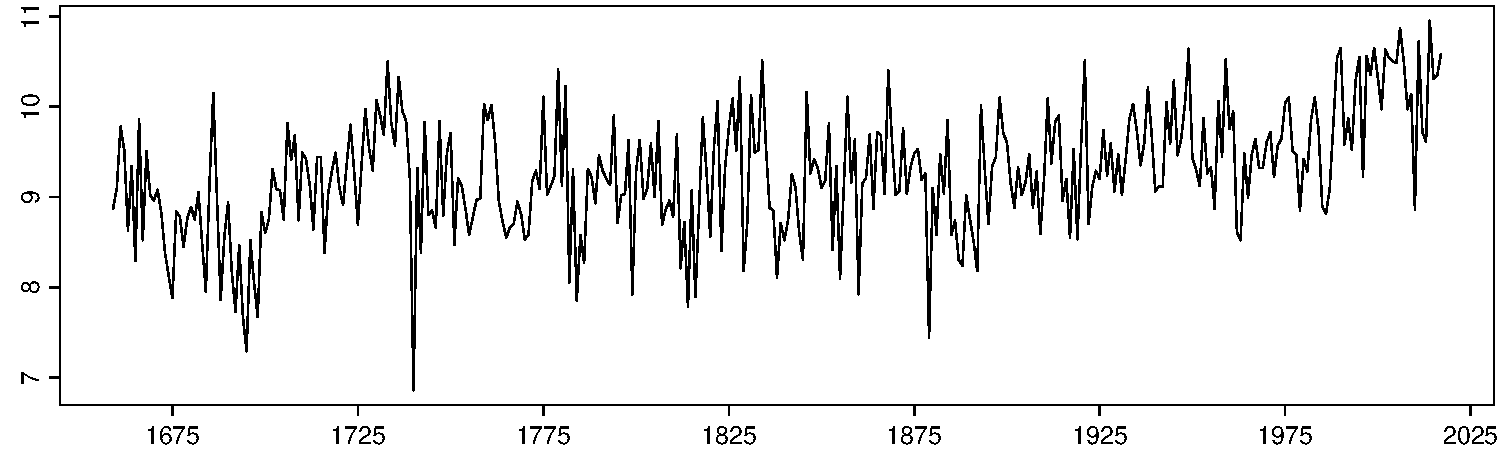
\includegraphics[width=0.9\textwidth]{Plots/temperature_data.pdf}
\vspace{0.2cm}

\caption{Yearly mean temperature in Central England for the time period from 1659 to 2017 measured in $^\circ$C.}\label{yearly_data}
\end{figure}


Let us first have a closer look at the situation where a single time series is observed. In this case, practitioners are interested in questions such as the following: Does the observed time series have a trend at all? If so, which are the time regions where there is a strong trend? Is the trend decreasing or increasing in these regions? As an example, consider the time series plotted in Figure \ref{yearly_data} which shows the yearly mean temperature in Central England from 1659 to 2017. Climatologists are very much interested in analysing the trending behaviour of temperature time series like this; see e.g.\ \cite{Benner1999} and \cite{Rahmstorf2017}. Among other things, they would like to know whether there is an upward trend in the Central England mean temperature towards the end of the sample as visual inspection might suggest. In Section \ref{sec-test-shape}, we develop a statistical procedure to approach questions like this. Specifically, we construct a method to test the null hypothesis that there is no time trend in the data. Importantly, the proposed method does not only allow to test whether the null hypothesis of no trend is violated. It also allows to identify, with a pre-specified statistical confidence, time regions where there is an upward or downward trend in the data. As regards the temperature time series in Figure \ref{yearly_data}, we can for example claim, with a statistical confidence of approximately 95\%, that there is some upward movement of the trend in the time period between ?? and ??. This is one of the results obtained from a detailed analysis of the time series as conducted in Section \ref{sec-data}. 


Let us now turn to the situation where multiple time series of the form \eqref{model2-intro} are observed. An important question in many applications is whether the time trends $m_i$ of the various time series are all the same. When some of the time trends are different, there may still be groups of time series with the same time trend. In this case, it is often of interest to estimate the unknown groups from the data. In addition, when two time trends $m_i$ and $m_j$ are not the same, it may also be relevant to know in which time regions they differ from each other. In Section \ref{sec-test-equality}, we construct statistical methods to approach these questions. In particular, we develop a test of the hypothesis that all time trends in model \eqref{model2-intro} are the same, that is, $m_1 = m_2 = \ldots = m_n$. Similar as above, our method does not only allow to test whether the null hypothesis is violated. It also allows to detect, with a given statistical confidence, which time trends are different and in which time regions they differ from each other. Based on our test method, we further construct a clustering algorithm which estimates groups of time series with the same time trend.


We develop our methods and the underlying theory step by step in Sections \ref{sec-method}--\ref{sec-test-equality}. In Section \ref{sec-method}, we introduce our methods in the context of a simple baseline case. We in particular discuss the problem of testing the simple hypothesis $H_0: m = 0$ in model \eqref{model1-intro}. In Sections \ref{sec-test-shape} and \ref{sec-test-equality}, we adapt the methods and theory to the test problems we are actually interested in. To construct our methods, we build on ideas from statistical multiscale testing as developed in \cite{ChaudhuriMarron1999,ChaudhuriMarron2000}, \cite{HallHeckman2000} and \cite{DuembgenSpokoiny2001} among others. Considering the hypothesis $H_0: m = 0$ in model \eqref{model1-intro}, our test procedure can be outlined roughly as follows: In a first step, we set up statistics $\widehat{\psi}_T(u,h)$ to test the hypothesis $H_0(u,h)$ that $m = 0$ on the interval $[u-h,u+h]$. In a second step, we aggregate these statistics $\widehat{\psi}_T(u,h)$ for a wide range of different intervals $[u-h,u+h]$. We thus construct a multiscale statistic which allows to test the hypothesis $H_0(u,h)$ simultaneously for many intervals $[u-h,u+h]$. A simple approach to aggregate the statistics $\widehat{\psi}_T(u,h)$ is to take their supremum $\sup_{(u,h) \in \mathcal{G_T}} \widehat{\psi}_T(u,h)$, where $\mathcal{G}_T$ denotes the set of points $(u,h)$ which are taken into account. As shown in the seminal work of \cite{DuembgenSpokoiny2001}, this approach is suboptimal in some sense. Following their lead, we define our multiscale statistic by $\widehat{\Psi}_T = \sup_{(u,h) \in \mathcal{G_T}} \{ \widehat{\psi}_T(u,h) - \lambda(h)\}$, where $\lambda(h)$ are additive correction terms. The idea behind this additively corrected supremum statistic is discussed in detail in Section \ref{sec-method}. 


In recent years, multiscale approaches have been developed for a variety of test problems. The general idea of all these approaches is to simultaneously consider a family of test statistics for a wide range of locations $u$ and scales or bandwidths $h$. This idea has been put to work in different ways, thus resulting in different multiscale test approaches. In the regression context, \cite{ChaudhuriMarron1999,ChaudhuriMarron2000} have developed the so-called SiZer method. 
% which has been extended in various directions; see for example \cite{KimMarron2006} and \cite{Huckemann2016} among others. 
\cite{HallHeckman2000} have constructed a multiscale test on monotonicity of a regression function. As already discussed above, \cite{DuembgenSpokoiny2001} have developed a multiscale approach which works with additively corrected supremum statistics. They derive theoretical results in the context of  a continuous Gaussian white noise model. Their theory can be extended in a fairly straightforward way to a nonparametric regression model $Y_t = m(t/T) + \varepsilon_t$ with i.i.d.\ Subgaussian errors $\varepsilon_t$. However, it is far from trivial to extend their theory to our setting, that is, to a nonparametric regression model $Y_t = m(t/T) + \varepsilon_t$ with a general weakly dependent error process $\{\varepsilon_t\}$. To derive our theoretical results, we come up with a proof strategy which is quite different from that of \cite{DuembgenSpokoiny2001}. This strategy is of interest in itself and may be applied to other multiscale test problems. It combines strong approximation results for dependent processes as developed in \cite{BerkesLiuWu2014} with anti-concentration bounds for Gaussian vectors as derived in \cite{Chernozhukov2015}. The details are described in Section \ref{sec-method}.


Our multiscale tests complement already existing tools for analysing nonparametric time trends. The test method developed in Section \ref{sec-test-shape} provides an alternative to dependent SiZer methods as introduced in \cite{Rondonotti2004} and \cite{Rondonotti2007}. Whereas the focus of these papers is mainly methodological, we back up our multiscale test by a complete asymptotic theory which characterizes its size and power properties. The multiscale test from Section \ref{sec-test-equality} is a valuable alternative to other procedures for testing equality of time trends. To the best of our knowledge, a multiscale test for the hypothesis $H_0: m_1 = m_2 = \ldots = m_n$ in model \eqref{model2-intro} has not been developed so far in the literature. However, there are other approaches to test for equality of time trends. \cite{Vogelsang2005} and \cite{Lyubchich2016}, for example, construct tests for comparing parametric time trends, whereas \cite{DegrasWu2012} develop an $L^2$-type test for comparing nonparametric trends. One of the advantages of our multiscale approach is that it is very informative: It does not only allow to test whether the null hypothesis is violated or not. It also gives information on where violations occur, in particular, which time trends are different and in which time regions they differ. It thus provides valuable additional information for practitioners. 


We complement the theoretical analysis of the paper by a simulation study and two application examples in Sections \ref{sec-sim} and \ref{sec-data}. The simulation study investigates the finite sample properties of the test methods and the clustering algorithm from Sections \ref{sec-test-shape} and \ref{sec-test-equality}. In the first application example, we examine the temperature time series from Figure \ref{yearly_data} with the help of the methods developed in Section \ref{sec-test-shape}. In the second, we analyse temperature time series measured at 34 different weather stations located in Great Britain. We in particular apply our procedure from Section \ref{sec-test-equality} to test whether the different time series have the same trend. 


